\chapter{ICE - CFD approach} \label{ch:ICETheory}

\section{Introduction}
The ICE (Implicit Compressible Eulerian) code for fluid simulations
in \Vaango uses a multi-material CFD approach designed to solve 
``full physics" simulations of dynamic fluid structure interactions 
involving large deformations and material
transformations (e.g., phase change).  ``Full physics" refers to
problems involving strong interactions between the fluid field and
solid field temperatures and velocities, with a full Navier Stokes
representation of fluid materials and the transient, nonlinear
response of solid materials.  These interactions may include chemical
or physical transformation between the solid and fluid fields.

The theoretical and algorithmic basis for the multi-material CFD
algorithm presented here is based on a body of work of several
investigators at Los Alamos National Laboratory, primarily Bryan
Kashiwa, Rick Rauenzahn and Matt Lewis.  Several reports by these
researchers are publicly available and are cited herein.  It is
largely through our personal interactions that we have been able to
bring these ideas to bear on the simulations described herein.

An exposition of the governing equations is given in the next section,
followed by an algorithmic description of the solution of those equations.
This description is first done separately for the materials in the Eulerian
and Lagrangian frames of reference, before details associated with the
integrated approach are given. 

\subsection{Governing Equations}\label{sec:governing_equations}
The governing multi-material model equations are stated and described, but
not developed, here.  Their development can be found in~\cite{Kashiwa2000}.
Here, our intent is to identify the quantities of interest, of which there
are eight, as well as those equations (or closure models) which govern their
behavior.  Consider a collection of $N$ materials, and let the subscript r
signify one of the materials, such that $\rmr = 1, 2, 3, \dots, N$.  In an
arbitary volume of space $V(\Bx,t)$, the averaged thermodynamic state of a
material is given by the vector $[M_\rmr, \Bu_\rmr, e_\rmr, T_\rmr, v_\rmr,
\theta_\rmr, \Bsig_\rmr, p]$, the elements of which are the $r$-material mass,
velocity, internal energy, temperature, specific volume, volume fraction,
stress, and the equilibration pressure.  The $r$-material averaged density is
$\rho_\rmr = M_\rmr/V$.  The rate of change of the state in a volume moving
with the velocity of $r$-material is:
\begin{align}
\frac{1}{V} \frac{D_\rmr M_\rmr}{Dt} &= \sum_{i=1}^N\Gamma_{\rmr\rms} \label{eq:eqmassr} \\
\frac{1}{V} \frac{D_\rmr}{Dt} (M_\rmr \Bu_\rmr) &=
  \theta_\rmr \Div{\Bsig} +
  \Div{\theta_\rmr(\Bsig_\rmr - \Bsig)} + 
  \rho_\rmr\Bg + 
  \sum_{i=1}^N \Bf_{\rmr\rms} + 
  \sum_{i=1}^N \Bu_{\rmr\rms}^+ 
  \Gamma_{\rmr\rms} \label{eq:eqmomr}\\ 
\frac{1}{V} \frac{D_\rmr}{Dt} (M_\rmr e_\rmr) &= -
  \rho_\rmr p \frac{D_\rmr v_\rmr}{ Dt} +
  \theta_\rmr\Btau_\rmr:\Grad{\Bu_\rmr} - 
  \Div{\Bj_\rmr} +
  \sum_{i=1}^N q_{\rmr\rms} +
  \sum_{i=1}^N h_{\rmr\rms}^+ 
  \Gamma_{\rmr\rms} \label{eq:eqenergyr}
\end{align}

Equations (\ref{eq:eqmassr}-\ref{eq:eqenergyr}) are the averaged model equations
for mass, momentum, and internal energy of $r$-material, in which $\Bsig$ is
the mean mixture stress, taken here to be isotropic, so that $\Bsig = -p\BI$
in terms of the hydrodynamic pressure $p$.  The effects of turbulence have
been explicitly omitted from these equations, and the subsequent solution,
for the sake of simplicity.  However, including the effects of turbulence
is not precluded by either the model or the solution method used here.

In Eq. (\ref{eq:eqmomr}) the term $\sum_{s=1}^{N}\Bf_{\rmr\rms}$ signifies
a model for the momentum exchange among materials.  This term results from
the deviation of the r-field stress from the mean stress, averaged, and is
typically modeled as a function of the relative velocity between materials
at a point. (For a two material problem this term might look like $\Bf_{12}
= K_{12}\theta_1\theta_2(\Bu_1 - \Bu_2)$ where the coefficient $K_{12}$
determines the rate at which momentum is transferred between materials).
Likewise, in Eq. (\ref{eq:eqenergyr}), $\sum_{\rms=1}^{N} q_{\rmr\rms}$
represents an exchange of heat energy among materials.  For a two material
problem $q_{12} = H_{12}\theta_1\theta_2(T_2 - T_1)$ where $T_\rmr$ is the
$r$-material temperature and the coefficient $H_{\rmr\rms}$ is analogous to a
convective heat transfer rate coefficient.  The heat flux is $\Bj_\rmr =
-\rho_\rmr b_\rmr \Grad{T_\rmr}$ where the thermal diffusion coefficient
$b_\rmr$ includes both molecular and turbulent effects (when the turbulence
is included).

In Eqs. (\ref{eq:eqmassr}-\ref{eq:eqenergyr}) the term $\Gamma_{\rmr\rms}$ is
the rate of mass conversion from s-material into $r$-material, for example,
the burning of a solid or liquid reactant into gaseous products.  The rate at which
mass conversion occurs is governed by a reaction model.  In Eqs. (\ref{eq:eqmomr})
and (\ref{eq:eqenergyr}), the velocity $\Bu_{\rmr\rms}^+$ and the enthalpy
$h_{\rmr\rms}^+$ are those of the s-material that is converted into $r$-material.
These are simply the mean values associated with the donor material.

The temperature $T_\rmr$, specific volume $v_\rmr$, volume fraction
$\theta_\rmr$, and hydrodynamic pressure $p$ are related to the $r$-material
mass density, $\rho_\rmr$, and specific internal energy, $e_\rmr$, by way
of equations of state.  The four relations for the four quantites $(T_\rmr,
v_\rmr, \theta_\rmr, p)$ are:
\begin{align}
e_\rmr &= e_\rmr(v_\rmr, T_\rmr) \label{eq:caloric} \\
v_\rmr &= v_\rmr(p, T_\rmr) \label{eq:thermal}
\end{align}
and
\begin{align}
\theta_\rmr &= \rho_\rmr v_\rmr \label{eq:thedef} \\
0 &= 1 - \sum_{i=1}^N\rho_\rms v_\rms \label{eq:mmeos}
\end{align}
Equations (\ref{eq:caloric}) and (\ref{eq:thermal}) are, respectively, the caloric
and thermal equations of state.  Equation (\ref{eq:thedef}) defines the volume
fraction, $\theta$, as the volume of $r$-material per total material volume,
and with that definition, Equation (\ref{eq:mmeos}), referred to as the
multi-material equation of state, follows.  It defines the unique value of
the hydrodynamic pressure $p$ that allows arbitrary masses of the multiple
materials to identically fill the volume $V$.  This pressure is called the
``equilibration'' pressure \cite{kashiwaICE94}.

A closure relation is still needed for the material stress $\Bsig_\rmr$.
For a fluid $\Bsig_\rmr = -p\BI + \Btau_\rmr$ where the deviatoric stress
is well known for Newtonian fluids.  For a solid, the material stress is the
Cauchy stress.  The Cauchy stress is computed using a solid constitutive
model and may depend on the the rate of deformation, the current state of
deformation ($\BE$), the temperature, and possibly a number of history
variables.  Such a relationship may be expressed as:
\begin{equation}
\Bsig_\rmr \equiv \Bsig_\rmr(\Grad{\Bu_\rmr}, \BE_\rmr, T_\rmr,~ \dots)
\label{eq:conslaw}
\end{equation}

The approach described here imposes no restrictions on the types of constitutive relations
that can be considered.  More specific discussion of some of the models
used in this work can be found in the section on ICE models.

Equations (\ref{eq:eqmassr}-\ref{eq:conslaw}) form a set of eight equations for
the eight-element state vector, \\ $[M_\rmr, \Bu_\rmr, e_\rmr, T_\rmr,
v_\rmr, \theta_\rmr, \Bsig_\rmr, p]$, for any arbitrary volume of space $V$
moving with the $r$-material velocity.  The approach described here uses the
reference frame most suitable for a particular material type.  As such,
there is no guarantee that arbitrary volumes will remain coincident for
materials described in different reference frames.  This problem is addressed
by treating the specific volume as a dynamic variable of the material state
which is integrated forward in time from initial conditions.  In so doing,
at any time, the total volume associated with all of the materials is given by:
\Beq
V_t = \sum_{r=1}^N M_\rmr v_\rmr
\Eeq
so the volume fraction is $\theta_\rmr = M_\rmr v_\rmr / V_t$ (which sums
to one by definition).  An evolution equation for the $r$-material specific
volume, derived from the time variation of Eqs. (\ref{eq:caloric}-\ref{eq:mmeos}),
has been developed in \cite{Kashiwa2000}.  It is stated here as:
%
\Beq
\frac{1}{V} \frac{D_\rmr}{Dt} (M_\rmr v_\rmr) =
  f_\rmr^{\theta} \Div{\Bu} +
  \left[v_\rmr \Gamma_\rmr -
  f_\rmr^{\theta} \sum_{i=1}^N
  v_\rms \Gamma_\rms \right]  +
  \left[\theta_\rmr
  \beta_\rmr \frac{D_\rmr T_\rmr}{Dt} -
  f_\rmr^{\theta} \sum_{i=1}^N
  \theta_\rms \beta_\rms \frac{D_\rms T_\rms}{Dt} \right] \, .
\label{eq:eqspvolr}
\Eeq
where 
\Beq
  f_\rmr^{\theta} = \cfrac{\theta_\rmr \kappa_\rmr}{\sum_{\rms =1}^N \theta_\rms\kappa_\rms}
\Eeq
and $\kappa_\rmr$ is the $r$-material bulk compressibility.

The evaluation of the multi-material equation of state (Eq. (\ref{eq:mmeos})
is still required in order to determine an equilibrium pressure that results
in a common value for the  pressure, as well as specific volumes that fill
the total volume identically.

A description of the means by which numerical solutions to the equations in
Section~\ref{sec:ICE:algorithm} are found is presented next.  This begins
with separate, brief overviews of the methodologies used for the Eulerian
and Lagrangian reference frames.  The algorithmic details necesssary for
integrating them to achieve a tightly coupled fluid-structure interaction
capability is provided in Sec.~\ref{ch:MPMICE}.

\section{Algorithm Description}\label{sec:ICE:algorithm}

The Eulerian method implemented here is a cell-centered, finite volume,
multi-material version of the ICE (for Implicit, Continuous fluid, Eulerian)
method \cite{harlowamsden68} developed by Kashiwa and others at Los Alamos
National Laboratory \cite{kashiwaCCICE94}.  ``Cell-centered'' means that all
elements of the state are colocated at the grid cell-center (in contrast to
a staggered grid, in which velocity components may be centered at the faces
of grid cells, for example).  This colocation is particularly important
in regions where a material mass is vanishing.  By using the same control
volume for mass and momentum it can be assured that as the material mass goes
to zero, the mass and momentum also go to zero at the same rate, leaving a
well-defined velocity.  The technique is fully compressible, allowing wide
generality in the types of problems that can be addressed.
 
Our use of the cell-centered ICE method employs time splitting: first,
a Lagrangian step updates the state due to the physics of the conservation
laws (i.e., right hand side of Eqs.~{\ref{eq:eqmassr}-\ref{eq:eqenergyr}}); this
is followed by an Eulerian step, in which the change due to advection is
evaluated.  For solution in the Eulerian frame, the method is well developed
and described in \cite{kashiwaCCICE94}.

In the mixed frame approach used here, a modification to the multi-material
equation of state is needed.  Equation (\ref{eq:mmeos}) is unambiguous when all
materials are fluids or in cases of a flow consisting of dispersed solid grains
in a carrier fluid.  However in fluid-structure problems the stress state of a
submerged structure may be strongly directional, and the isotropic part of the
stress has nothing to do with the hydrodynamic (equilibration) pressure $p$.
The equilibrium that typically exists between a fluid and a solid is at the
interface between the two materials: there the normal part of the traction
equals the pressure exerted by the fluid on the solid over the interface.
Because the orientation of the interface is not explicitly known at any
point (it is effectively lost in the averaging) such an equilibrium cannot
be computed.

The difficulty, and the modification that resolves it, can be understood by
considering a solid material in tension coexisting with a gas.  For solid
materials, the equation of state is the bulk part of the constitutive response
(that is, the isotropic part of the Cauchy stress versus specific volume and
temperature).  If one attempts to equate the isotropic part of the stress
with the fluid pressure, there exist regions in pressure-volume space for
which Eq. (\ref{eq:mmeos}) has no physical solutions (because the gas pressure
is only positive).  This can be seen schematically in Fig.~\ref{fig:vpfig}, which
sketches equations of state for a gas and a solid, at an arbitrary temperature.

\begin{figure}[htbp!]
  \centering
  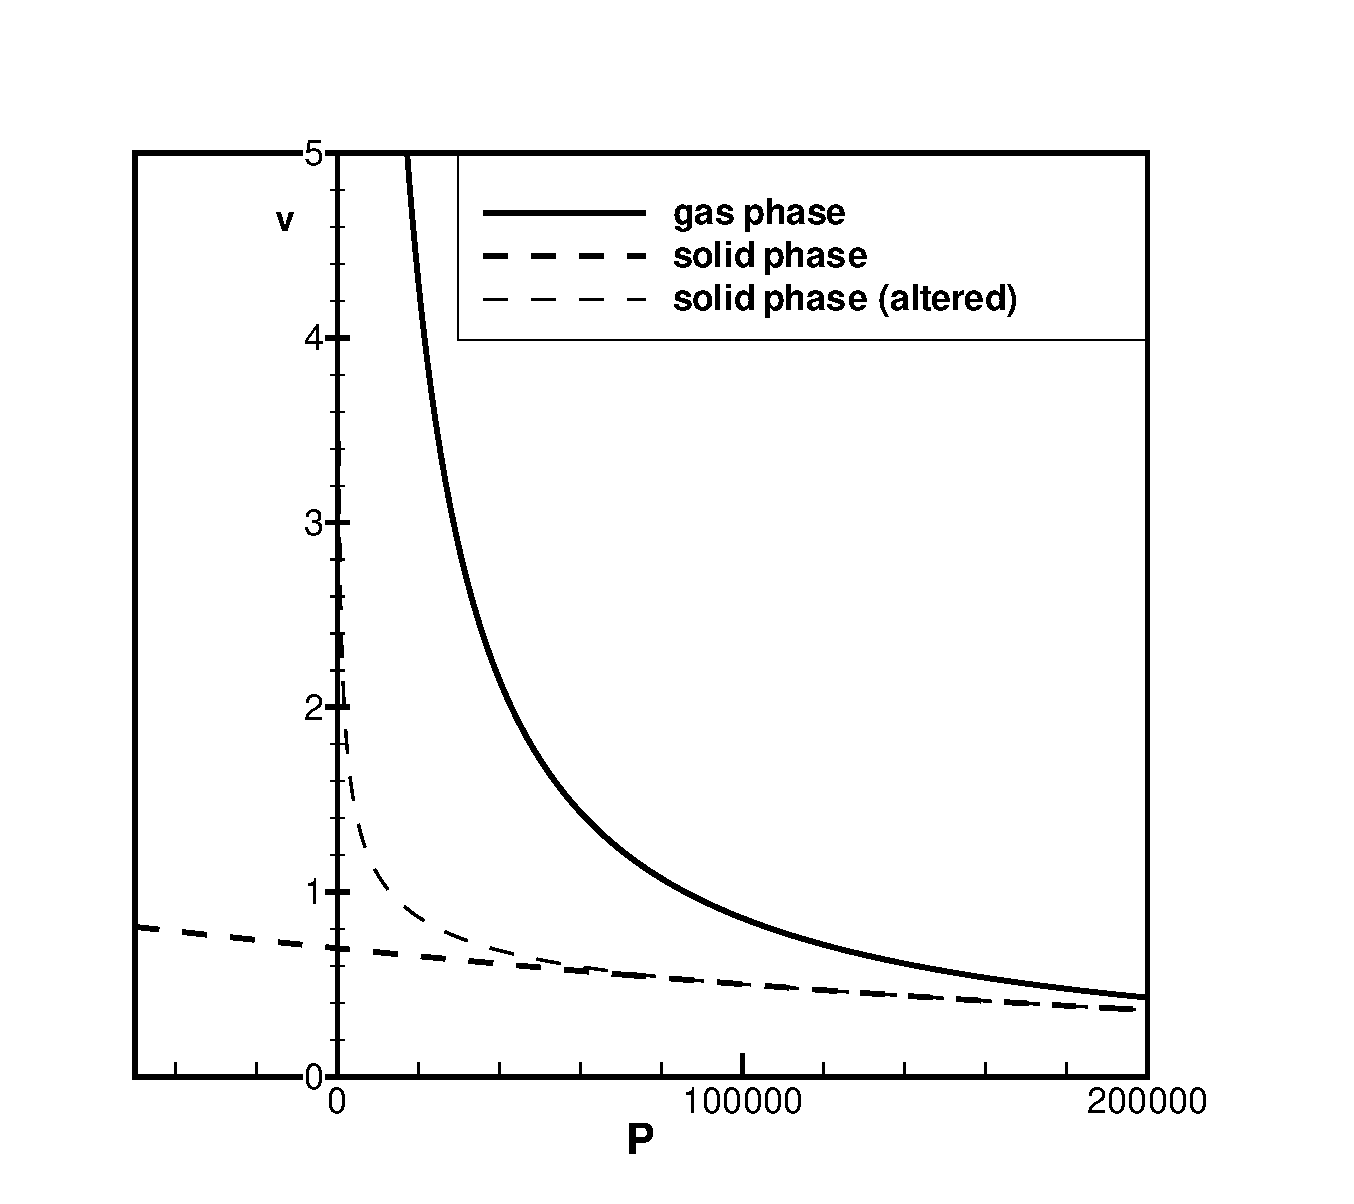
\includegraphics[width=0.5\textwidth]{Figs/mpmice/v_p_new.pdf}
  \caption{Specific volume \textit{vs} pressure for a gas phase material 
          and a solid phase material.  Light dashed line reflects an 
          altered solid phase equation of state to keep all materials
          in positive equilibration pressure space.}
  \label{fig:vpfig}
\end{figure}

Recall that the isothermal compressiblity is the negative slope of the
specific volume versus pressure.  Embedded structures considered here are
solids and, at low pressure, possess a much smaller compressibility than
the gasses in which they are submerged.  Nevertheless the variation of
condensed phase specific volume can be important at very high pressures,
where the compressibilities of the gas and condensed phase materials can
become comparable (as in a detonation wave, for example).  Because the speed of
shock waves in materials is determined by their equations of state, obtaining
accurate high pressure behavior is an important goal of our FSI studies.

To compensate for the lack of directional information for the embedded
surfaces, we evaluate the solid phase equations of state in two parts.
Above a specified postive threshold pressure (typically 1 atmosphere),
the full equation of state is respected; below that threshold pressure, the
solid phase pressure follows a polynomial chosen to be $C^1$ continuous at the
threshold value and which approaches zero as the specific volume becomes large.
The effect is to decouple the solid phase specific volume from the stress when
the isotropic part of the stress falls below a threshold value.  In regions
of coexistence at states below the threshold pressure, $p$ tends to behave
according to the fluid equation of state (due to the greater compressibility)
while in regions of pure condensed phase material $p$ tends rapidly toward
zero and the full material stress dominates the dynamics as it should.

